\section{Modelo Cinemático}

O sistema modelado consiste em um robô com tração diferencial,  
que se movimenta em um plano bidimensional (x, y) e é controlado por dois motores  
de corrente contínua, conforme representado na Figura \ref{fig:robot_model}.
\begin{figure}[h]
    \centering
    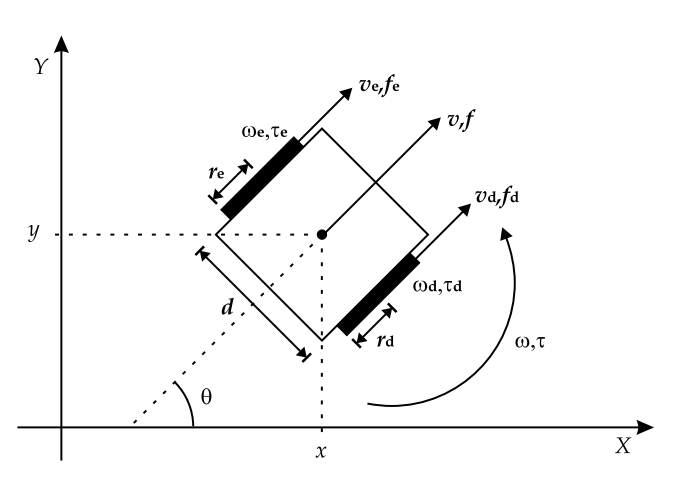
\includegraphics[width=0.8\textwidth]{figures/robot_model.png}
    \caption{Modelo do robô com tração diferencial}
    \label{fig:robot_model}
\end{figure}

A seguinte nomenclatura é utilizada:

\begin{itemize}
    \item $v$, $\omega$: velocidade linear e angular do robô;
    \item $\omega_d$, $\omega_e$: velocidade angular das rodas;
    \item $v_d$, $v_e$: velocidade linear das rodas;
    \item $r_d$, $r_e$: raio das rodas;
    \item $d$: distância entre as rodas;
    \item $(x, y)$, $\theta$: coordenadas e orientação do robô no plano;
    \item $f$, $\tau$: força e torque aplicados sobre o robô;
    \item $f_d$, $f_e$: forças aplicadas nas rodas;
    \item $\tau_d$, $\tau_e$: torques aplicados nas rodas;
\end{itemize}

\subsection{Relação entre Velocidades, Posição e Orientação}

Em \cite{vieira2005controle}, o modelo cinemático é descrito  
por um sistema de equações que relaciona a velocidade  
linear e angular do robô com a velocidade angular das rodas.  
Para encontrar o modelo começamos definindo as velocidades tangenciais das rodas:
\begin{equation}
v_e = \omega_e r_e
\qquad  
\qquad
v_d = \omega_d r_d
\end{equation}

A partir da velocidade linear e angular do robô,  
podem-se relacionar as velocidades tangenciais das rodas:
\begin{equation}
v_e = v - \frac{d}{2} \omega
\qquad  
\qquad
v_d = v + \frac{d}{2} \omega
\label{eq:velocities}
\end{equation}
\begin{figure}[h]
    \centering
    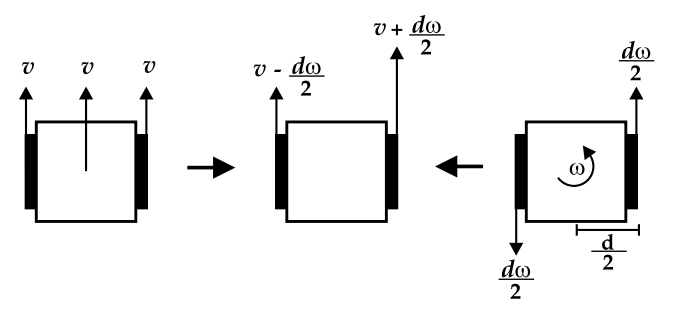
\includegraphics[width=0.55\textwidth]{figures/robot_composition.png}
    \caption{Composição do modelo cinemático}
    \label{fig:robot_composition}
\end{figure}

Ou, ao contrário, a partir das velocidades das rodas, podemos relacioná-las com a velocidade do robô:
\begin{equation}
v = \omega_d \frac{r_d}{2} + \omega_e \frac{r_e}{2} 
\qquad
\qquad
\omega = \omega_d \frac{r_d}{d} - \omega_e \frac{r_e}{d}
\label{eq:cinematic_model}
\end{equation}
\begin{figure}[h]
    \centering
    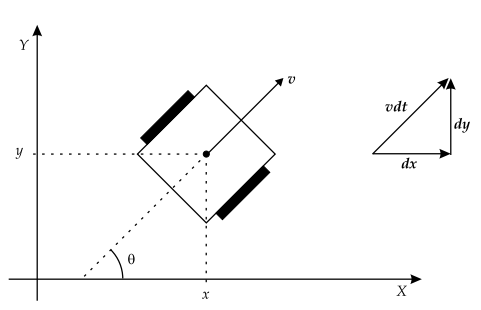
\includegraphics[width=0.55\textwidth]{figures/robot_coordinates.png}
    \caption{Coordenadas do robô no plano}
    \label{fig:robot_coordinates}
\end{figure}

Ao relacionar os movimentos cinemáticos a deslocamentos incrementais  
em um plano bidimensional, como na Figura \ref{fig:robot_coordinates},  
tem-se que a velocidade do robô pode ser expressa como:
\begin{equation}
\begin{cases}
\dot{x} = v \cos(\theta) \\
\dot{y} = v \sin(\theta) \\
\dot{\theta} = \omega
\end{cases}
\label{eq:cinematic_velocity}
\end{equation}